%
% tests.tex
%
% Copyright (C) 2021 by SpaceLab.
%
% FloripaSat-2 Documentation
%
% This work is licensed under the Creative Commons Attribution-ShareAlike 4.0
% International License. To view a copy of this license,
% visit http://creativecommons.org/licenses/by-sa/4.0/.
%

%
% \brief Test plan and results.
%
% \author Gabriel Mariano Marcelino <gabriel.mm8@gmail.com>
%
% \institution Universidade Federal de Santa Catarina (UFSC)
%
% \version 0.1.0
%
% \date 2021/01/21
%

\chapter{Test Plan and Results} \label{ch:test-plan}

The FloripaSat-2 test plan is structured into four phases: Module tests, FlatSat, Engineering integration, and Flight integration. This plan is summarized in the \autoref{tab:test-plan} and includes the components under test for each phase. 

\begin{table}[!h]
    \begin{center}
        \begin{tabular}{ll}
            \toprule[1.5pt]
            \textbf{Phase}    & \textbf{Components}       \\
            \midrule
            Module tests             & OBDH module \\
                                     & EPS module \\
                                     & TTC module \\
                                     & BATC4 board \\
                                     & IIP boards \\
                                     & PC104-ADPT boards \\
                                     & ACS components (simulation) \\
                                     & Mechanical (CAD assessment) \\
            \midrule
            FlatSat                  & Satellite core (OBDH+EPS+TTC+BATC4) \\
                                     & Satellite core + GRS \\
                                     & Satellite core + Payloads \\
                                     & Satellite core + Payloads + GRS \\
                                     & Satellite (long-term evaluation) \\
            \midrule
            Engineering integration  & Mechanical assembly (repeated when required) \\
            (clean room preferable)  & Satellite core + Payloads + GRS \\
                                     & Satellite (long-term evaluation) \\
                                     & Satellite + Solar Panels \\
                                     & Preliminary environmental tests \\ 
            \midrule
            Flight integration       & Mechanical assembly (flight components) \\
            (clean room mandatory)   & Satellite (short-term evaluation) \\
                                     & Satellite + Antenna (deployment) \\
                                     & Mechanical reassembly for flight \\
                                     & Satellite (long-term evaluation) \\
                                     & Qualification environmental tests \\ 
            \bottomrule[1.5pt]
        \end{tabular}
        \caption{Test plan phases and tested components.}
        \label{tab:test-plan}
    \end{center}
\end{table}

This section focus on providing an overview of the planned testing workflow and a description of the strategies approached to accomplish the mission objectives. The module tests focus on the individual modules operation and behavior, in which a general template is provided in this document and each module applies it for their needs. The FlatSat phase is the first modules integration in a debug platform to validate the system from a development perspective (described with more details in \cite{flatsat}). Finally, the engineering integration is the final development campaign aiming to validate the system from a mission perspective and the flight integration is the actual CubeSat assembly using the flight components and final assessments to prepare the satellite for launch. The integration details, procedures and qualification proccess are described with more depth in the \autoref{ch:ait}. % maybe it will be splitted in a separated document


\section{Module tests}

The first phase is the foundation for the satellite, consolidating the base design for each subsystem and shaping their relations. Therefore, several techniques were employed to ensure a solid test strategy: several inspections of the boards design and manufacturing quality; manual experimental assessments of various hardware electrical, mechanical and behavioral parameters; remotely automated tests using a continuos integration (CI)\nomenclature{\textbf{CI}}{\textit{Continuos Integration.}} approach; semi-automated tests using a hardware-in-the-loop (HIL)\nomenclature{\textbf{HIL}}{\textit{Hardware-In-the-Loop.}} strategy; simulations; and CAD models assessment.

\subsection{Workflow}

The following topics lists the template workflow used to create the procedures for each subsystem. Each module documentation has its own test chapter describing the process in detail, from procedures to success criteria.

% \item [\footnotesize{XX-00}] Text 
\subsubsection{Visual Inspection} 
\begin{enumerate} \setlength\itemsep{-0.3em}
    \item Packaging quality assessment
    \item Board manufacturing and assembly quality
    \item 3D model comparison
    \item Layers marker
    \item Labels (schematics comparison) 
    \item High resolution photos for documentation
\end{enumerate}

\subsubsection{Mechanical Inspection}
\begin{enumerate} \setlength\itemsep{-0.3em}
    \item Board dimensions and mounting holes positioning
    \item Board weight measurement
\end{enumerate}

\subsubsection{Integration Inspection}
\begin{enumerate} \setlength\itemsep{-0.3em}
    \item Check connectors pinout against the documentation (not schematics)
    \item Check connectors positioning (if applicable)
\end{enumerate}

\subsubsection{Electrical Inspection}
\begin{enumerate} \setlength\itemsep{-0.3em}
    \item Solder shorts
    \item Missing components
    \item Lifted pins
    \item Poor soldering
    \item Swapped components
    \item Components partnumber
    \item Components polarity (schematic comparison)
    \item Components defined to not be soldered (DNP)
\end{enumerate}

\subsubsection{Electrical Testing}
\begin{enumerate} \setlength\itemsep{-0.3em}
    \item Continuity test
    \item Power up procedures (check LEDs and testpoints)
    \item Average input power consumption measurement
    \item Average output power source measurement (if applicable) 
    \item Power tracks temperature (if applicable)
    \item Simple signal integrity (if applicable)
\end{enumerate}

\subsubsection{Functional Testing}
\begin{enumerate} \setlength\itemsep{-0.3em}
    \item Run a simple test code (if applicable) 
    \item Run the system code (if applicable and available) 
    \item Check the system hardware self-test flags (if applicable and available) 
    \item Monitor basic LEDs behavior (if applicable) 
    \item Monitor the debug serial port logs (if applicable)
\end{enumerate}

\subsubsection{Module Testing}
\begin{enumerate} \setlength\itemsep{-0.3em}
    \item Run simulations and review results (if applicable)
    \item Review operation behavior against the documentation (if applicable)
    \item Review features and requirements fulfillment
    \item Review communication buses configuration and protocol (if applicable)
    \item Review data packages, power buses and control signals
    \item Review and evaluate operation edge cases
    \item Run remote automated code tests (if applicable)
    \item Run system test codes in the board (if applicable)
    \item Run latest stable code version, monitor logs and qualify behavior (if applicable)
\end{enumerate}

\subsection{Continuos Integration}

In order to detect errors and bugs in the early stages of development, a continuos integration workflow was setup for automated firmware tests focusing in small scope verfications (i.e., unit tests). Instead of executing the code in the target processor, the tests are executed remotely in a host computer through the usage of an unit testing framework, called ``cmocka'' \cite{cmocka}. This tool allows to abstract the inherent hardware dependencies of embedded systems to enable firmware tests without errors introduced by hardware problems (exection in a consolidated platform, the computer), which provides an optimal behavioral assessment of the code implementations. This approach not only support remote testing, but promote continuos test execution, which is essencial to detect erros and architectural issues. The integration of these procedures is powered by ``GitHub Actions'' \cite{gh-actions}, which provides a host machine and a dashboard inside the same environment of the already used version control, source distribution and management tool.

The unit tests follows a layered structure accordingly with the firmware layers. This is used alongside mockups (i.e., interfaces that abstract what the layer receive as input without having to implement the underlying functionality), which allows independency between the layers and abstract the actual hardware dependencies with an emulated behavior.

\subsection{Hardware-In-the-Loop}

In the context of embedded systems, many errors are caused by hardware issues and limitations. Then, it is important to assess the system operation running in the actual hardware platform. The hardware-in-the-loop strategy bring this elements in a more contolled and automated test environment. The idea is to execute the firmware in the board with an emphasis on evaluating the general behavior and operation flow, since there are several log messages used to report the system current status or action across the execution.


\section{Flatsat}

To test all modules during the development of the projet, a flatsat platform was developed. The FlatSat Platform is a testbed for CubeSat PCB modules. FlatSats enable easier, faster and a secure method for testing subsystens independently while been integrated in a flat design before going to integration on a CubeSat form factor. The PCB can support up to 7 modules, all PC-104 pins are interligated to flexibilize its use, only the particularity connection between modules need to be be taken into account. One PC-104 has inverted pinout, the board also makes it possible to have two seperate power supplies, a UART to USB converter for 4 modules, kill-switches activation though SPDTs, Remove Before Flight (RBF) pin header, connector for charging batteries and SMA connectors for antennas. A picture of the flatsat board can be seen in \autoref{fig:flatsat-top}.

\begin{figure}[!ht]
    \begin{center}
        \includegraphics[width=\textwidth]{figures/flatsat_top_image}
        \caption{Top view of the flatsat board.}
        \label{fig:flatsat-top}
    \end{center}
\end{figure}

Besides the hardware platform itself, during the FlatSat phase, a setup is used with the same structure as the hardware-in-the-loop strategy herein mentioned. Instead of using logs of one board, the analysis is performed from the perspective of all modules under test, which provides an evaluation of a complete system (satellite). More information about the Flatsat hardware platform and procedure details can be found in \cite{flatsat}.


\section{Engineering integration}

The engineering model integration is the final development campaign since it connects the satellite design in the actual CubeSat form factor, allowing the assessment not only of the system from a behavioral perspective (as performed in the FlatSat), but also from the application and mission point of view. This is achieved due to additional elements (e.g., actual mechanical frame), environmental tests and execution of use cases. Also, it is possible to early evaluate electrical, mechanical and behavioral compliance fulfillment.

During this phase, the FlatSat process and test methodology is repeated in a condensed manner, since the system was already tested and some preliminary procedures can be skipped. The mechanical assembly is performed several times, until the design and the related documentation are settled. The environmental tests are a simplified version of the final process for qualification, but open opportunities for early assessments and more destructive procedures. Also, the long-term testing provides a comprehensive knowledge of the satellite reliability and robustness. Further details are provided in the \autoref{ch:ait} section.


\section{Flight integration}

The flight model integration performs the last arrangements before launch in a clean room, including: evaluation assembly with all final parts; last test campaign, the same as executed in the engineering integration; reassembly with definitive parts, placement and resin; qualification environmental tests; and flight-ready procedures (packaging, transport and pre-launch).

LIT\nomenclature{\textbf{LIT}}{\textit{Laboratório de Integração e Testes.}}

\cite{marcelino2021}


\section{Preliminary Results}


\subsubsection{Output Power of the Radio Modules}

The output power of the radio modules can be measured using a spectrum analyzer, as can be seen in the picture of \autoref{fig:rf-output-power-test}.

\begin{figure}[!ht]
    \begin{center}
        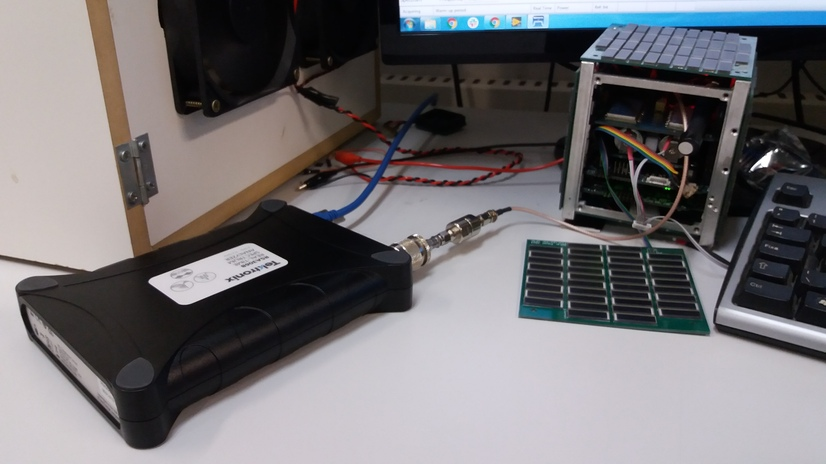
\includegraphics[width=\textwidth]{figures/rf-output-power-test.jpg}
        \caption{RF output power test with the radio modules connected to a spectrum analyzer.}
        \label{fig:rf-output-power-test}
    \end{center}
\end{figure}

The measured values for the beacon and downlink transmitters are available in Figures \ref{fig:beacon-power} and \ref{fig:downlink-power} respectively.

\begin{figure}[!ht]
    \begin{center}
        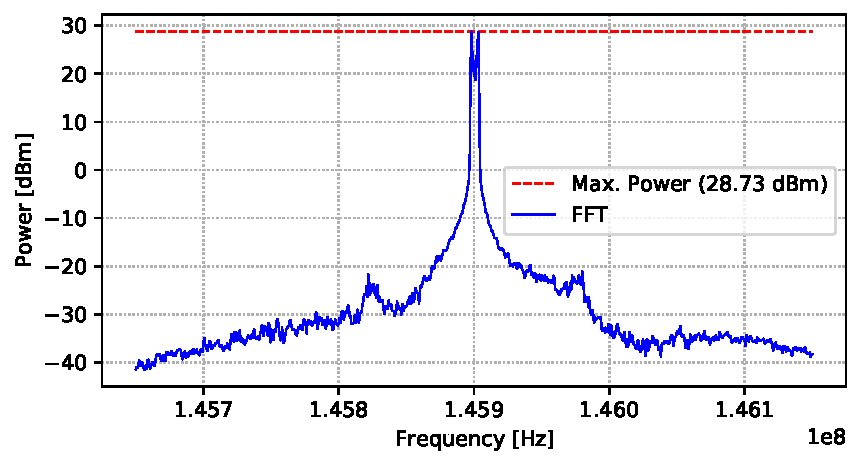
\includegraphics[width=\textwidth]{curves/beacon_output_power.pdf}
        \caption{Output power of the beacon radio.}
        \label{fig:beacon-power}
    \end{center}
\end{figure}

\begin{figure}[!ht]
    \begin{center}
        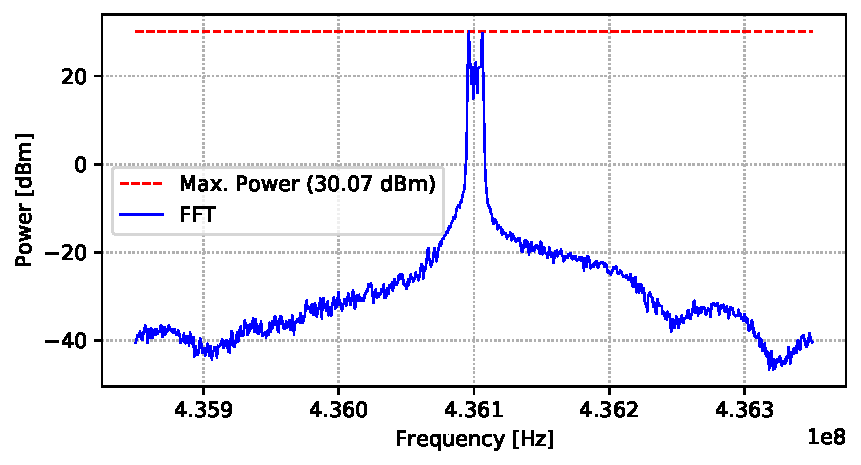
\includegraphics[width=\textwidth]{curves/downlink_output_power.pdf}
        \caption{Output power of the downlink radio.}
        \label{fig:downlink-power}
    \end{center}
\end{figure}
